\documentclass[conference]{IEEEtran}
%\IEEEoverridecommandlockouts
% The preceding line is only needed to identify funding in the first footnote. If that is unneeded, please comment it out.
\usepackage{cite}
\usepackage{amsmath,amssymb,amsfonts}
\usepackage{algorithmic}
\usepackage{graphicx}
\usepackage{textcomp}
\usepackage{xcolor}
\usepackage{float}
\graphicspath{ {./} }
\usepackage{listings}
\usepackage{color}
\usepackage{hyperref}

\definecolor{codegreen}{rgb}{0,0.6,0}
\definecolor{codegray}{rgb}{0.5,0.5,0.5}
\definecolor{codepurple}{rgb}{0.58,0,0.82}
\definecolor{backcolour}{rgb}{0.95,0.95,0.92}

% came from the ANSI escape sequence color table as implemented by Ubuntu
% used for colorizing the ls-description paragraph
\definecolor{folder-blue}{RGB}{0,111,184}
\definecolor{file-green}{RGB}{57,181,74}

\lstdefinestyle{mystyle}{
	backgroundcolor=\color{backcolour},   
	commentstyle=\color{codegreen},
	keywordstyle=\color{magenta},
	numberstyle=\tiny\color{codegray},
	stringstyle=\color{codepurple},
	basicstyle=\footnotesize,
	breakatwhitespace=false,         
	breaklines=true,                 
	captionpos=b,                    
	keepspaces=true,                 
	numbers=left,                    
	numbersep=5pt,                  
	showspaces=false,                
	showstringspaces=false,
	showtabs=false,                  
	tabsize=2
}

\lstset{style=mystyle}

% what does this do?  i commented it out and can't tell any difference -misha
\def\BibTeX{{\rm B\kern-.05em{\sc i\kern-.025em b}\kern-.08em
    T\kern-.1667em\lower.7ex\hbox{E}\kern-.125emX}}

\begin{document}

\title{CSci487 Penetration Testing Project: AILEE}

\author{\IEEEauthorblockN{Grant Haataja}
\IEEEauthorblockA{\textit{UND Computer Science} \\
Grand Forks, ND, USA \\
grant.haataja@und.edu}
\and
\IEEEauthorblockN{David Wilson}
\IEEEauthorblockA{\textit{UND Computer Science} \\
Grand Forks, ND, USA \\
david.andrew.wilson@und.edu}
\and
\IEEEauthorblockN{Michael Turnbull}
\IEEEauthorblockA{\textit{UND Computer Science} \\
Monroe, NH, USA \\
michael.turnbull@und.edu}
}

\maketitle

\begin{abstract}
This document details the planning, development, and workings of the penetration testing game AILEE, created as a final project for CSCI 487 Penetration Testing class at the University of North Dakota.
\end{abstract}

%\tableofcontents

%\begin{IEEEkeywords}
%component, formatting, style, styling, insert
%\end{IEEEkeywords}

\section{Introduction}
For this project on penetration testing topics, a hacking simulation game was created. The premise of the game is as follows: the user plays the role of a penetration-testing AI software named AILEE, which stands for Artificial Intelligence Linux Exploit Environment. The game takes place exclusively in a Linux-style terminal environment, with a limited arsenal of commands for the player to use. As the player progresses through the game and “learns” as an AI, the commands available for use increase. Throughout the game, the player is given typed instructions and information from the AI’s administrator to assist in learning. 

There are two targets to hack in this demo, although there is much potential for expansion. The game uses simulated port scanning, vulnerability scanning, exploitation, and other penetration testing tools to mimic real-life penetration testing methods. Additionally, the game features a storyline with three possible endings, depending on player actions. Special care was taken to handle proper sequence of events.

\section{Investigation}

\subsection{Planning the Project}

Before beginning the development of the game, a suitable platform to run the environment needed to be found. The website Repl.it was decided upon, due to their extensive language support and the ability for multiple people to work simultaneously and have all changes automatically saved to the cloud. \cite{b1} The “Multiplayer” mode, as this feature was called, still had a lot of bugs, so forking the project and saving work manually was still necessary, but overall it made the development of AILEE much smoother. 

Python3 was selected as the programming language of choice, due to its ease of scripting and strong object-oriented nature. The various classes corresponding to different aspects of the game and environment would be programmed separately, as well as Python scripts for each command available to the player, and every storyline event that could be run. The original plan was for there to be three different targets for the player to hack, but due to time limitations the scope was decreased to two targets.
    
To enable smooth graphics for the intro screen and the game’s ending events, the Python Curses library was referenced and used extensively. \cite{b2} This provided the ability to control keyboard input while text displayed on the screen or the ending event graphics played, to increase the smoothness of gameplay. 

\section{Project Description}

\subsection{Intro Screen}\label{AA}
For the graphics of the intro screen for the game, ASCII art was used to spell the word AILEE, along with a selection for New Game or Exit. The user can move between the selection using the up or down arrow keys and choose by pressing the enter key. Selecting Exit will cause the terminal session within Repl.it to exit and the game will have to be run again, selecting New Game creates a new session and runs the game. 

In addition to these, pressing the up arrow six times in a row will show a hidden third selection, Skip Dialog. This will run the game without displaying any of the instructions and information from the administrator to AILEE, and was very useful for testing the game during development. This mode is not explained or mentioned in the game, as it is not recommended to play without reading the dialogue.

The intro screen makes use of the Python curses library to allow smooth use of the arrow keys keyboard input and prevent buggy graphics.

\subsection{Starting the Game}
Upon choosing New Game, the user watches as the administrator logs into their account and launches AILEE.exe to start a new shell. After the shell loads, the first event triggers and text displays on the screen to inform the user what is going on. The administrator gives a brief explanation, and then the user is free to experiment with the Linux-style terminal environment. The terminal runs in the Shell class, (in tandem with the Game and DoStory classes), which supports multiple terminals on various computers. The code for the Shell class is as follows:

\lstinputlisting[language=Python]{shell.py}

The user is encouraged to try out the various possible commands, which can be displayed using the \textit{help} command. The story continues after the user has ran ten commands, (they can be the same or different commands, it doesn't matter).

\begin{figure}[h]
    \centerline{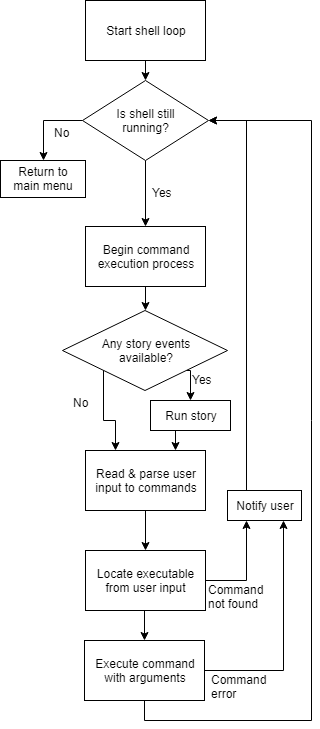
\includegraphics[scale=0.7]{shellloop.png}}
    \caption{Shell flow diagram}
    \label{fig:shell-flow}
\end{figure}

\subsection{Gameplay and Commands}
As the game progresses, the user will utilize the available penetration testing tools to gain access to the target computers. There are tools for finding IP addresses, port scanning, vulnerability scanning, exploitation, password cracking, and connecting through the ftp file sharing network. Generally, some of the commands require the results from running other commands in order to be run successfully. 

In particular, the \texttt{exploit} command is extremely useful for gaining access to other computers.  This command is similar to the Metasploit framework, commonly used in real-life penetration testing.  In the game, as the player uncovers exploits in different computers with the \texttt{vscan} command, those exploits are added to a global database of exploits which the user can then pick from in the \texttt{exploit} command.  Exploits are specific to a port on a computer, and if correctly used, will successfully open a new shell on the target computer.

\lstinputlisting[language=Python]{exploit.py}

Above is the code for the \textit{exploit} command in the game. In terms of options, it does not compare to the Metasploit framework, but the goal was to create it to feel similarly in the terminal environment.

\begin{figure}[h]
	\centerline{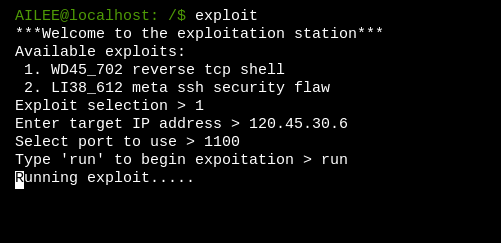
\includegraphics[scale=2]{exploit-pic}}
	\caption{Running the \textit{exploit} executable}
	\label{fig:exploit-pic}
\end{figure}

First, the user enters the number corresponding to the exploit they wish to run. Then, the target IP address is entered, followed by the specific port, and finally the command 'run' must be entered and the exploitation software will attempt to gain access to the target (Fig. \ref{fig:exploit-pic}) 

\begin{figure}[h]
	\centerline{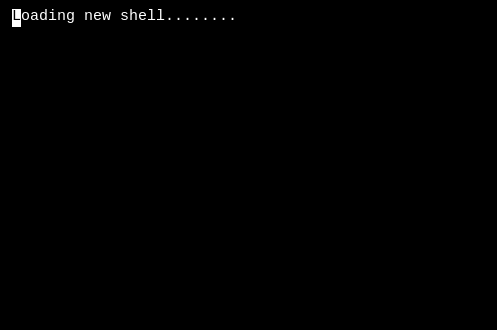
\includegraphics[scale=2]{loading-new-shell}}
	\caption{Gaining a shell on target machine}
	\label{fig:loading}
\end{figure}

If the exploit is successful, the screen will clear and the words "Loading new shell...." will appear on the screen with increasing dots as the shell loads (Fig. \ref{fig:loading})

\begin{figure}[h]
	\centerline{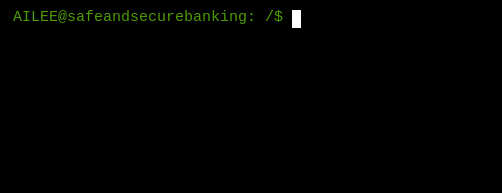
\includegraphics[scale=2]{access-granted}}
	\caption{A new shell on an exploited target}
	\label{fig:access}
\end{figure}

Once the shell loads, the name of the computer exploited will be shown before the \texttt{/\$} symbol where commands are typed (Fig. \ref{fig:access}).

Most of the other commands play an important role in the game, with a few exceptions that were included for comedic value.

\subsection{Events and Storyline}

The story development of the game is controlled by event scripts that are triggered at specific times. Running the events in the proper order is critical for the game to play as planned. The first event is run immediately after the game loads its first shell on the localhost computer. Each event after that has a condition that must be met to trigger it. The second event runs after ten commands have been run, the third event runs after the \textit{pscan} command runs, and so on. Each event runs instructions for the user that should allow them to trigger the next event and progress in the game.

\lstinputlisting[language=Python]{event3.py}

This is how the scripts for the events are written, implementing a custom-built "typewriter" function created to display text to the screen word by word as if it were typed, and using a blue color to differentiate it from the rest of the game text. 

\begin{figure}[h]
	\centerline{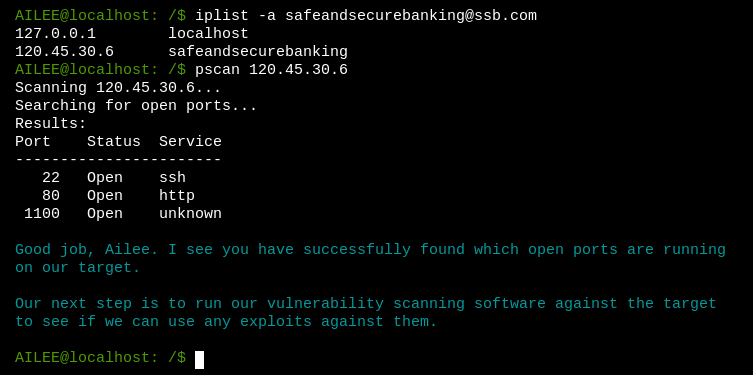
\includegraphics[scale=1.39]{event3}}
	\caption{The dialogue for event 3}
	\label{fig:event3}
\end{figure}

This is the text for the third event (Fig. \ref{fig:event3}), which triggers after the user runs the command \textit{pscan} against the first target IP address.

\begin{figure}[h]
    \centerline{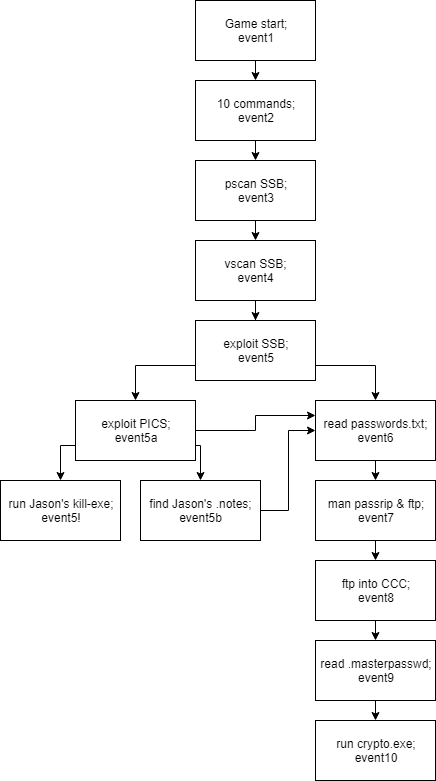
\includegraphics[scale=0.5]{gameflow.png}}
    \caption{The sequence of events in play order}
    \label{fig:gameplay-sequence}
\end{figure}

There are three special events that do not trigger in a normal play-through of the game. These events will only trigger if the player thinks for themselves and uses information found in the game creatively and without instruction from the administrator. Interestingly, if the user follows the instructions without diverging on their own, they will lose the game during the final hack. The only way to win is by finding what the information leads to and changing the fate of the game before attempting to exploit the final target.

\subsection{Computers and Filesystems}
AILEE uses a filesystem structure that feels like a Linux terminal. There are a total of four computers in the game, localhost (AILEE's home computer), the two targets, and one other computer. Each computer has a unique filesystem, with directories and files. As time was limited, the \textit{bin} and \textit{log} directories were left empty on all computers, but the \textit{home} directories all have files in them that either pertain to the gameplay or exist for comedic value or storyline development.

To navigate the filesystems, the traditional Linux commands \textit{ls} and \textit{cd} are used, as well as the commands \textit{read} and \textit{run}, which display file text and run executable files, respectively. 

\lstinputlisting[language=Python]{filesystem.py}

This is the code for the structure and mechanics of the computer filesystems. 
Similar to Linux, both files and folders have and use discrete permissions, 
marking certain files as readable, writable, and executable.  While there are not yet any
provisions for editing/creating files in-game\footnote{The \texttt{gcc} command
creates a file \texttt{a.out}, which promptly throws a segmentation fault.},
the permissions architecture is in place for adding future file-editing
utilities.

Executable files are created from a separate filesystem constructor.  Each
executable file simply is a \texttt{File} object with the executable bit set in
its permissions object, and the file contents are pure Python code that executes
when the file is run via the \texttt{run} command.  To verify that arbitrary
code is not run (which would break the game), executable files compare hashes
from creation to runtime to and will not run if the contents have been
altered.

\begin{figure}[htbp]
	\centerline{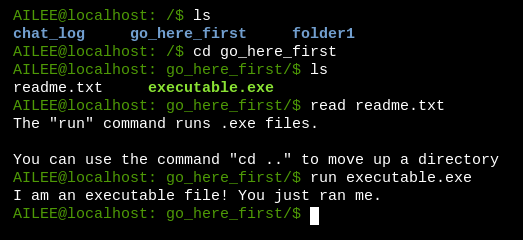
\includegraphics[scale=2]{filesystem-example}}
	\caption{Filesystem navigation}
	\label{fig:ls-command}
\end{figure}

Directories are colored light blue, executables are light green, and regular files are white.  Because of the permissions associated with each file and directory, and the fact that \texttt{File} and \texttt{Directory} objects are implemented as separate classes, there are no special requirements to file/folder names or attributes.  However, due to the difficult implementation of a directory tree, the \textit{ls} command cannot be given a path argument as in real life, and thus can only be used in the current directory.

\section{Conclusion}
In summary, this project dives into many core concepts and facets of penetration testing, and simulates them to feel like the real-world counterparts. Many of the commands that simulate complicated software are coded creatively to look realistic even though they only work in the specific instances inside the game. AILEE is a demo, and there is much opportunity to expand the game into something far more complex and realistic if enough time and energy was dedicated to doing so.

\begin{thebibliography}{00}
\bibitem{b1} Repl.it, ``The world's leading online coding platform,'' repl.it. [Online]. Available: \url{https://repl.it/site/features}. [Accessed: 02-May-2019].

\bibitem{b2} A. M. Kuchling and E. S. Raymond, ``Curses Programming with Python,'' Curses Programming with Python - Python 3.7.3 documentation. [Online]. Available: \url{https://docs.python.org/3/howto/curses.html}. [Accessed: 02-May-2019].
\end{thebibliography}

\end{document}